\section{Damara Benedikta (1174012)}
\subsection{Pengertian SIG}
SIG atau system informasi geografis merupakan sebuah system informasi yang berbasis computer dimana dirancang untuk dapat bekerja mengolah data yang memiliki informasi spasial. Didalam system tersebut dapat melakukan pengecekan, pengintegrasian, manipulasi,analisa dan menampilkan data secara spasial yang mereferensikan kondisi bumi

\subsection{Sejarah SIG}
Pada 35000 tahun yang lalu para pemburu diprancis mereka menggambar hewan pemangsa dan juga garis yang dipercya sebagai rute dari migrasi hewan hewan tersebut. Itu merupakan sebuah catatan awal pada system informasi geografis. 
awal abad 20 dimulailah pengembangan litografi foto yang mana peta dipisahakan beberapa lapisan (layer). Perkembangan perangkat keras komputer yang dipacu oleh penelitian senjata nuklir membawa aplikasi pemetaan menjadi multifungsi pada awal tahun 1960-an.
Sehingga pada tahun 1967 sebagai awal pengembangan  dari SIG yang  diterapkan di Ottawa, Ontario oleh Departemen Energi, Pertambangan dan Sumber Daya. SIG sendiri dikembangkan oleh Roger Tomlinson, yang kemudian disebut CGIS (Canadian GIS – SIG Kanada), yang memiliki kegunaan sebagai penympanan penganalisa dan pengolahan data yang telah dikumpulkan untuk inventarisasi tanah di Kanada.
Canadian GIS adalah system pertama yang berasal dari perbaikan aplikasi pemetaan yang dikembangkan oleh Roger Tomlinson yang disebut juga sebagai bapak SIG. Canadian GIS  sangat membutuhkan waktu lama dalam proses pengembangannya dan tidak dapat bersaing dengan aplikasi pemetaan yang lain. 
SIG berkembang seiring dengan ditemukannya komputer. Pada era perang dunia ke II, banyak kebutuhan  yang memicu perkembangan SIG guna membantu pemrosesan data untuk memenuhi kebutuhan militer.
Jack Dangermond yang belajar di labolatorium komputer grafik Harvard menemukan program Environmental Systems Research Institute (ESRI) Pada tahun 1969,  yang kemudian dikembangkan dan mampu menghasilkan software ArcInfo dan ArcView. Tahun 1970, SIG pertama kali digunakan oleh Roger Tomlinson dan Duane Marble. Dan juga pada tahun  1980 dan 1990, aplikasi SIG digunakan untuk berbagai kepentingan yang merambah ke banyak negara dengan berbagai model. Beberapa jenis aplikasi komersial dipublikasikan selama periode ini, seperti ArcView, MapInfo, ArcInfo, SMALLWORLD, SPANS GIS, INTERGRAPH dan PAMAP GIS.

\subsection{Koordinat}
Sitem koordinat merupakan posisi sebuah titik dimana dinyatakan dengan menggunakan 2 dimensi atau tiga dimensi yang mengacu pada sebuah system koordinat. Dalam sebuah titik koordinat mengacu pada 3 parameter dibawah: 
\begin{itemize}
	\item Lokasi Titik Nol dari Sistem Koordinat
Posisi suatu titik di permukaan bumi umumnya ditetapkan dalam/terhadap suatu sistem koordinat terestris. Titik nol dari sistem koordinat terestris ini dapat berlokasi di titik pusat massa bumi (sistem koordinat geosentrik), maupun di salah satu titik di permukaan bumi (sistem koordinat toposentrik).

	\item Orientasi dari Sumbu-sumbu Koordinat
	Dalam posisi tiga-dimensi (3D) suatu titik  yang dinyataan dalam suatu system koordinat geosentrik. Dimana tergantung jug pada setip parameternya. Jenis koordinat ada 2 yaitu koordinat kartesian dengan sumbu x,y dan z. 
	\begin{itemize}
	\item Latitude
	garis lintang mengarah dari khatulistiwa (0) ke kutub selatan, atau khatulistiwa ke kutub utara (sudut 0-90 dan 0 -90)

	\item Longitude
	merupakan garis bujur yang berarti sebuah  garis horizontal seperti dari khatulistiwa. Pada sudut 0 (Greenwich) ke arah Hawai adalah dari angka 0-180 drajat, sedangkan kebalikannya dari angka 0 ke -180

\end{itemize}
\end{itemize}
Titik 0 dimulai dari garis negara Inggris. Mengarah ke Indonesia akan menjadi angka positif. Kebalikannya koordinat Longitude minus adalah arah kebalikan.


\subsection{Data Geospasial}
Data Geospasial merupakan sebuah data mengenai lokasi geografis , dimensi ukuran atau karakteristik objek alam maupun objek buatan manusia yang berada dibawah ataupun diatas permukaan bumi . Pembahasan:
\begin{itemize}
	\item Satu
	Data sistem penentuan posisi global (GPS). Data GPS dikumpulkan melalui sistem navigasi radio berbasis satelit dan darat. Smartphone berkemampuan GPS dapat memberikan lokasi seseorang.

	\item Dua
	Data Penginderaan jauh melibatkan instrumen khusus yang menangkap data yang bisa diubah menjadi bentuk digital. Seperti halnya pada Satelit, pemindai, dan sistem radar adalah salah satu  contoh dari instrumen ini. Contoh lain dari penginderaan jauh adalah foto udara.

\end{itemize}
Dengan adanya data geospasial kita bisa melihat ruas jalan yang padat ataupun macet. Dengan mengetahui keadaan ini, bihak berwenang seperti polisi laku kintas dapat melakukan penanganan seperti pengalihan arus ke jalur alternatif atau pemberlakuan jalan satu arah.  

\subsection{Link}
\href {https://youtu.be/3P1zRqXBvx4}{klik disini}
\subsection{Plagiarism}
\begin{figure}[H]
	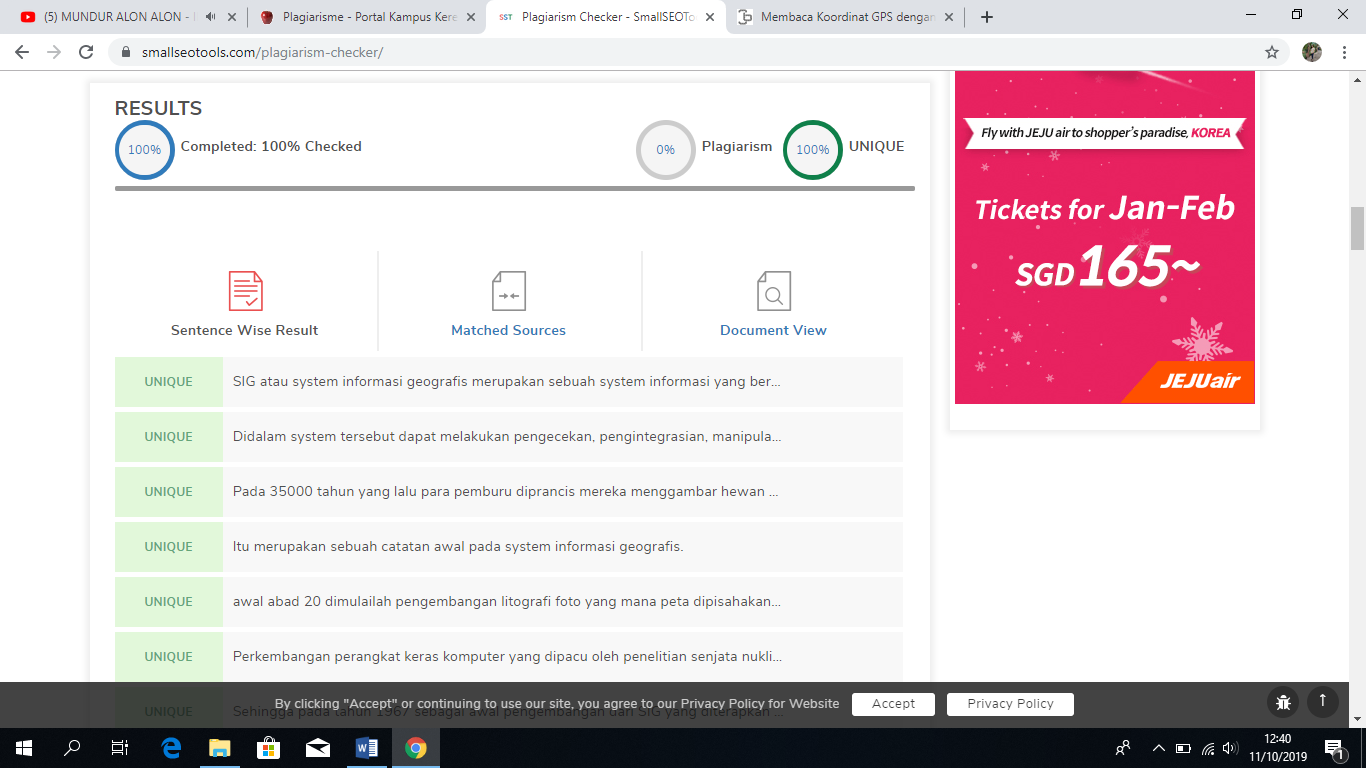
\includegraphics[width=4cm]{figures/1174012/gb.png}
	\centering
	\caption{Bukti}
\end{figure}